La sesión analizada contó con un total de 70 senadores,
pertenecientes a 27 partidos políticos, distribuidos del
siguiente modo (Figura \ref{fig-distrib-senators}):

\begin{figure}[h!]
\centering
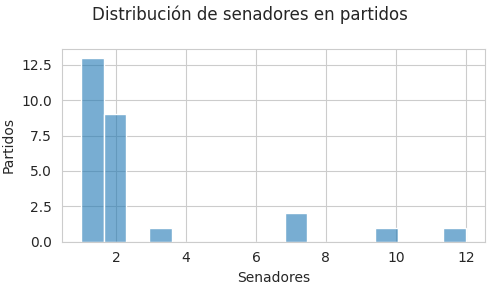
\includegraphics[scale=0.7]{../visualizations/distrib_histplot_senators_parties.png}
\caption{Distribución de senadores en partidos políticos y en provincias.}
\label{fig-distrib-senators}
\end{figure}

Aquí vemos que solo uno de los partidos (Frente de todos) cuenta con 12
senadores; también uno solo (Alianza frente para la victoria) es
representado por 10 senadores; dos partidos (Alianza cambiemos y
Juntos por el cambio) cuentan con 7 senadores, y el resto de los
partidos tienen entre 3, 2 y un senador.
En cuanto a las provincias (24 en total), todas tienen 3 senadores
exceptuando a Tucumán y a La Rioja, que tienen solo 2.

La figura \ref{fig-distrib-vote} nos muestra además que la intención
de voto no guarda una relación unívoca con los partidos a los cuales los
senadores representan. A excepción de los partidos que cuentan con un único
senador, la mayoría cuenta con senadores que votaron a favor y senadores
que votaron en contra de la ley para el acceso al aborto. Aquí también
es posible ver que un senador del Frente Justicialista se abstuvo de votar,
mientras que dos senadores, uno de Cambiemos Fuerza Cívica Riojana y uno de
Frente Unidad Justicialista San Luis, estuvieron ausentes en la votación.

\begin{figure}[h!]
\centering
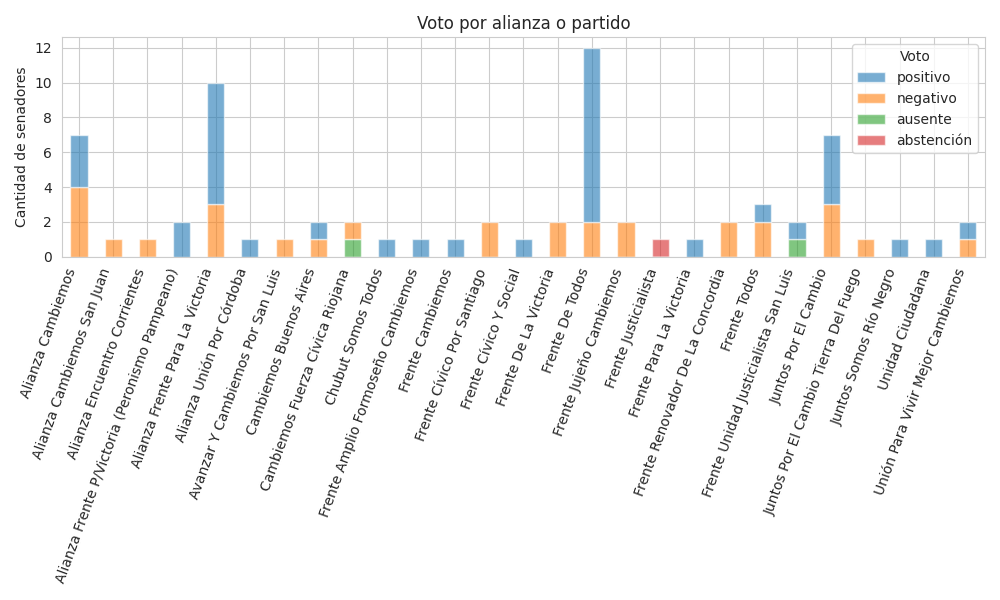
\includegraphics[scale=0.48]{../visualizations/senators_vote_by_party.png}
\caption{Distribución de votos en los distintos partidos políticos.}
\label{fig-distrib-vote}
\end{figure}

En cuanto a las intervenciones discursivas, observamos que, en promedio, se emitiieron
2.87 discursos por senador, con un desvío de 6.23 y una mediana de 1, coincidente además
con la moda. Estas medidas de centralidad, incluyen 9 senadores que no intervinieron en
la sesión, 7 de ellos votaron en contra de la despenalización del aborto; uno, a favor,
y uno estuvo ausente durante la votación. La figura \ref{fig-distrib-speech} muestra esta
distribución global y también discriminada por intención de voto.\todo{explicar un poco esto}

\begin{figure}[h!]
    \centering
    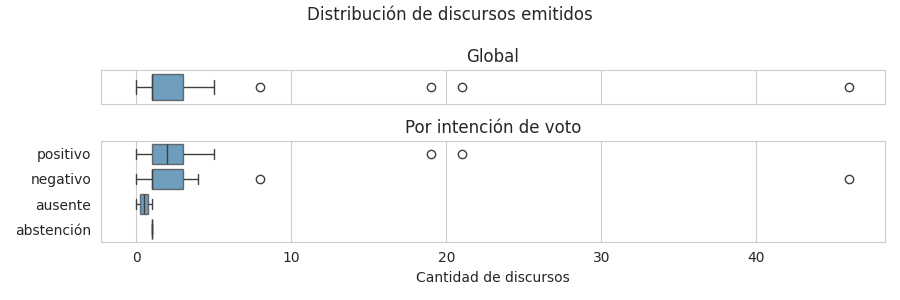
\includegraphics[scale=0.5]{../visualizations/speech_by_vote.png}
    \caption{Distribución de votos en los distintos partidos políticos.}
    \label{fig-distrib-speech}
\end{figure}

\begin{table}[ht]
\centering
\begin{tabular}{ |c|c|c|c|c| }
    \hline
    Voto & Media & Desvío & Mediana & Moda \\
    \hline\hline
    Abstención & 1.00 & 0.00 & 1.00 & 1 \\
    \hline
    Ausente & 0.50 & 0.71 & 0.50 & 0 \\
    \hline
    Negativo & 3.03 & 8.43 & 1.00 & 1 \\
    \hline
    Positivo & 2.92 & 4.26 & 2.00 & 1 \\
    \hline
\end{tabular}
\caption{Medidas de centralidad de la cantidad de discursos emitidos}
\label{table-tokens}
\end{table}

%
%
%% con qué voy a seguir?
%% - métricas/gráficos de diversidad de tokens y tokens únicos
%% - explicar que esto podría ser un problema
%% - explicar que para el análisis al nivel de la oración elegí probar con stemmizado y lemmatizado
%% - el stemmer y el lemma ya es cuestión de la metodología
%    
\begin{table}[h!]
\begin{center}
\begin{tabular}{ |c|c|c|c| }
\hline
Tokens & Media & Mediana & Desvío Estándar \\
\hline\hline
Totales & 811.65 & 636.12 & 714.79 \\
\hline
Únicos & 296.47 & 254.25 & 238.68 \\
\hline
\end{tabular}
\caption{M\'etricas univariadas de la cantidad de tokens}
\label{table-tokens}
\end{center}
\end{table}
